\documentclass[a4paper]{article}
\usepackage{graphicx}
\usepackage[utf8]{inputenc}
\usepackage[english, serbian]{babel}

\title{UseCase: Pregled radne verzije izdanja časopisa}
\date{10.11.2018.}
\author{Dimitrije}

\begin{document}

\maketitle

\begin{itemize}
    \item Akter: Glavni urednik časopisa
    \item Kratak opis: Glavni urednik vrši pregled radne verzije tekućeg izdanja časopisa.
    \item Osnovni tok događaja:
        \begin{enumerate}
            \item Glavni urednik zahteva od sistema pregled radne verzije tekućeg izdanja časopisa.
            \item Sistem prikazuje radnu verziju tekućeg izdanja časopisa.
        \end{enumerate}
    \item Alternativni tok događaja:
        \begin{enumerate}
            \item  (2) Sistem ne prikazuje radnu verziju. Glavni urednik pokušava ponovo da izvrši korak 1. Ukoliko ne uspe, obraća se administratoru časopisa.
        \end{enumerate}
\end{itemize}

\begin{figure}
    \centering
    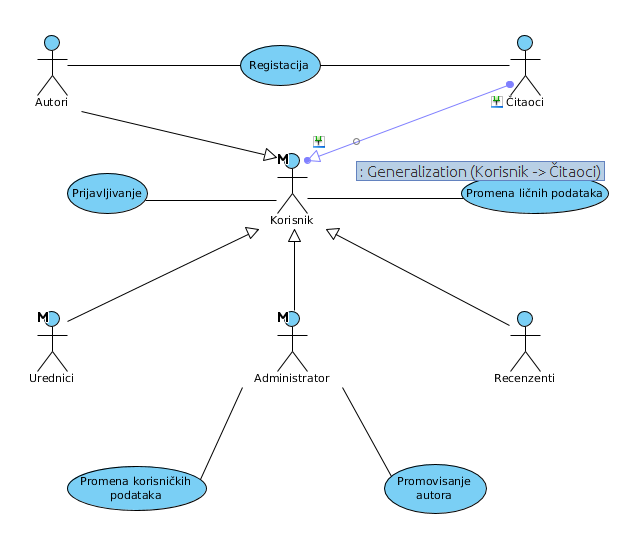
\includegraphics[width=\linewidth]{usecasePrijavljivanje.png}
    \caption{UseCase screenshot}
    \label{fig:my_label}
\end{figure}


\end{document}
